\documentclass{beamer}
% \usepackage[brazil]{babel}
\usepackage[utf8]{inputenc}
\usepackage{fancybox}
\title[Teaching]{Teaching}
%\subtitle[short version]{}
%\date{}
\author[Sivaram Ambikasaran]{Sivaram Ambikasaran}
\institute[IITM]{Indian Institute of Technology Madras}
\usetheme{Madrid}


 
\usecolortheme{owl}
\setbeamercolor{normal text}{fg=orange}
\usebeamercolor*{normal text}
\begin{document}
\frame{\titlepage}


\begin{frame}{Teaching Philosophy}
	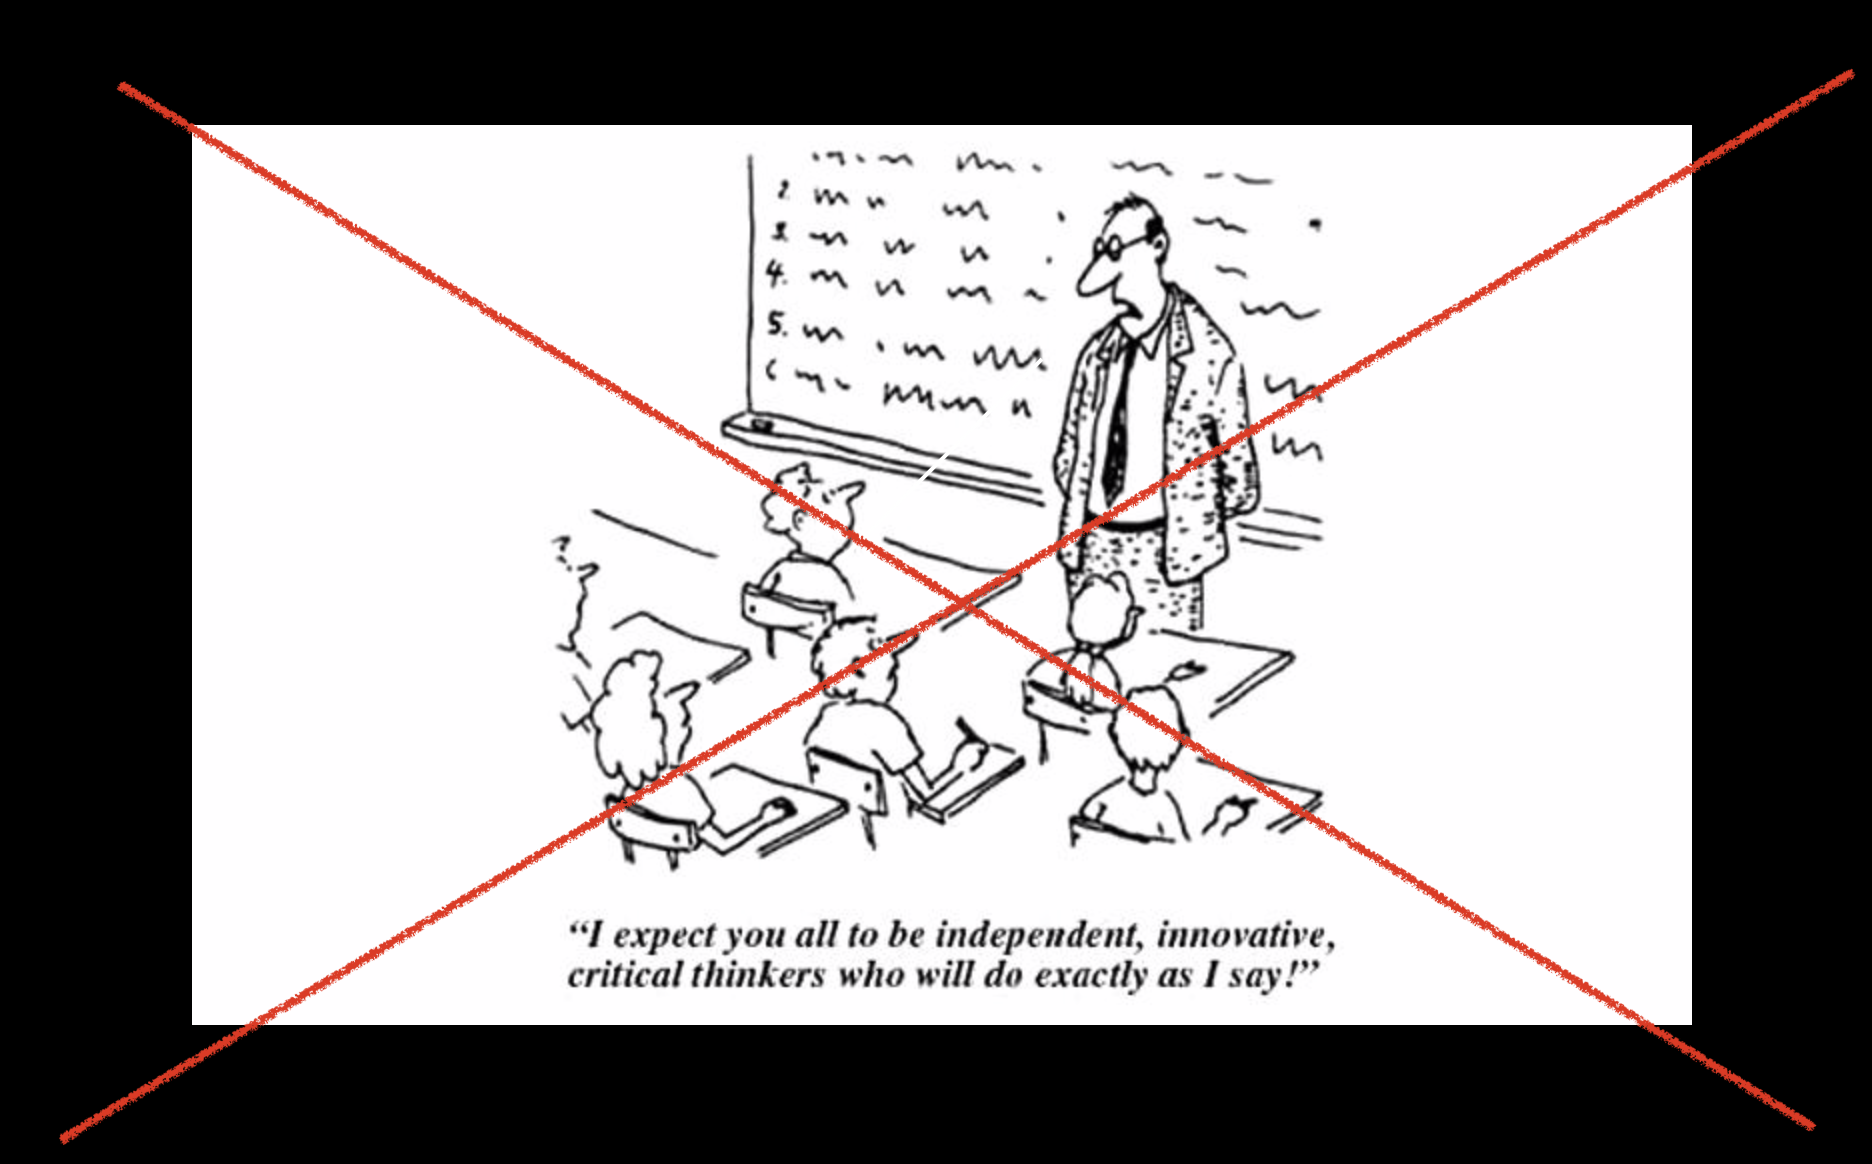
\includegraphics[width=\textwidth]{./images/Comic_Teaching.png}
\end{frame}

\begin{frame}[c]{Teaching Philosophy}
	\begin{center}
	\Huge{Teacher, Professor?}\\
	\pause
	\vspace{2em}
	\Huge{I am an {\color{cyan}educational} {\color{magenta}rockstar}}
	\end{center}
\end{frame}

\begin{frame}[c]{Teaching Philosophy}
	\LARGE
	\begin{center}
		``Intellectually entertain students and make them learn"\\
	\vspace{1em}
	``Don’t try to teach, try to make the students learn”\\
	\vspace{1em}
	``Try to figure things out along with the students"
	\end{center}
\end{frame}

\begin{frame}[c]{Teaching Philosophy}
	\LARGE
	\begin{itemize}
		\item
		Spend the first lecture on motivation
		\item
		Why, What and How?
		\item
		Numerical Linear Algebra
		\begin{itemize}
			\item
			The \$25,000,000,000 Eigenvector: Linear algebra behind google
			\item
			The Smart Money’s on Numerical Analysts
		\end{itemize}
	\end{itemize}
\end{frame}

\begin{frame}[c]{Teaching Philosophy}
	\LARGE
	Adopt latest technologies in teaching
	
\includegraphics[scale=0.1]{./images/Github.png}
	
\includegraphics[scale=0.1]{./images/Jupyter.png}
	
\includegraphics[scale=0.1]{./images/AutoGradr.png}
	
\includegraphics[scale=0.1]{./images/JPlag.png}
\end{frame}

\begin{frame}{Example: Finite Precision Computation}
	\LARGE
	Solving recurrence
	$$a_{n+1} = 10a_n - 9a_{n-1}$$
	with $a_0 = a_1 = 2.95$
\end{frame}

\begin{frame}{Polynomial Interpolation \& Approximation}
	\LARGE
	Interpolate/Approximate
	$$f(x) = \dfrac1{1+25x^2}$$
	Weierstrass approximation theorem
\end{frame}

\begin{frame}{MonteCarlo to compute $\pi$}
	\LARGE
	$1/\sqrt{N}$ convergence of MonteCarlo methods
\end{frame}

\begin{frame}{Teaching Philosophy}
	\LARGE
	To heighten the understanding of concepts
	\begin{itemize}
		\item
		Live computational and mathematical demonstrations
		\item
		Proofs and more importantly examples/counterexamples
	\end{itemize}
	Enables students to understand the details as well as to get the bird's eye view of the entire landscape
	Students get confidence to see that programming can be simple and fun to play around.
\end{frame}
\end{document}